\chapter{Evaluation}

\section{Cost Benchmark}

This section aims to provide a rough guidance on expected cost for each variant of the smart contract.

Actual costs will vary over time as the Ether-to-USD exchange rate as well as the network gas price will change. It is also dependant of the desired transaction confirmation speed. To avoid this section becoming inaccurate in the future, only the amount of gas consumed is benchmarked. The actual cost can be calculated using the cost model described in chapter 5.

\subsection{Variant 1}
For variant 1, a benchmark script was created\footnote{The source code can be found under \texttt{v1-gas-benchmark.js}. The benchmark can be executed with \texttt{node index v1-gas-benchmark --count=5}.}. The benchmark calculates the cumulative gas spent on contract creation and IP address insertion. Two cases were calculated: For the worst case, each IP address was inserted in a separate transaction. For the best case, reports were bundled into one transaction. The benchmark was executed in both cases for 1 IP address, then 2 IP addresses and so forth up to 20 IP addresses. The resulting costs are displayed in Figure \ref{fig:v1-gas-cost}.

\begin{figure}[H]
\centering
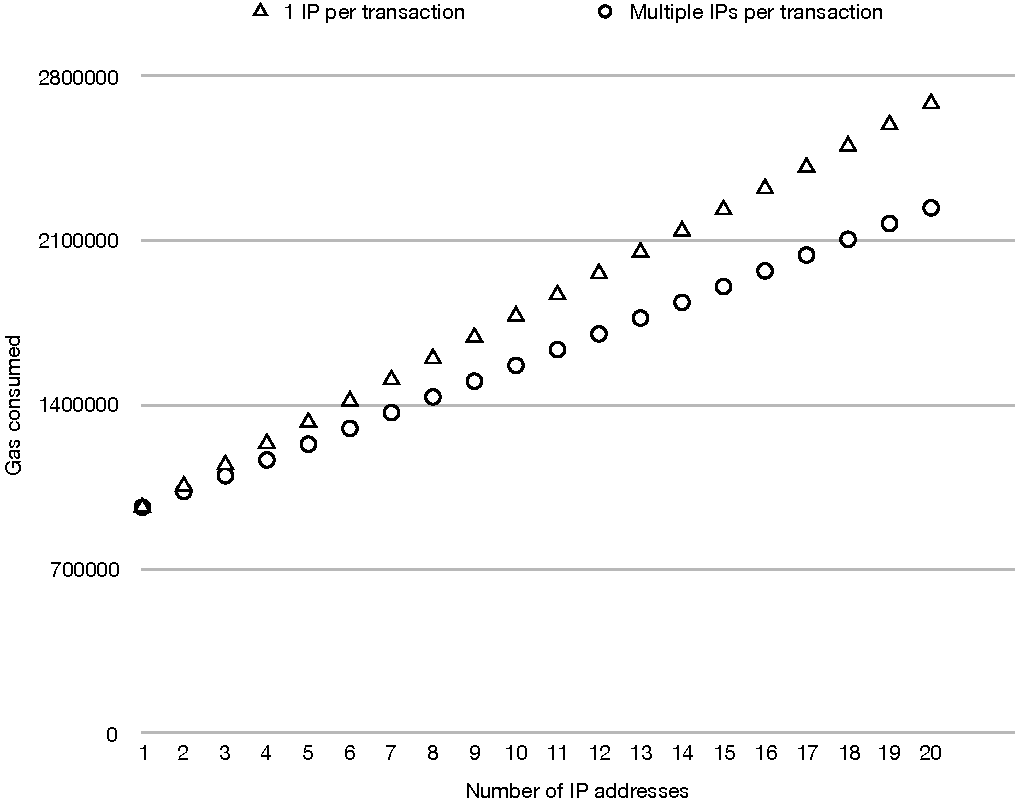
\includegraphics[width=0.7\textwidth]{v1-gas-cost.pdf}
\caption{Gas cost incurred using variant 1}
\label{fig:v1-gas-cost}
\end{figure}

For only a few reports, the major cost is the initial deployment of the contract, costing approximately 858'000 gas. Adding reports costs approximately 150'000 - 200'000 gas each.
It can be observed that bundling reports into one transaction can save 24\% of the gas cost beyond the initial cost (this is however not always practical, as new reports have to be accumulated before they can be bundled, which might make the insertion slower).

Even in the best case, the costs grow linearly ($\mathcal{O}(n)$) as new reports are added. This makes variant 1, as predicted, expensive and unsuitable for big amounts of IP addresses.

\subsection{Variant 2}
For variant 2 (web resource pointer), the cost benchmark of the Solidity contract is trivial, however additional infrastructure is needed whose cost is hard to quantify.

For the gas cost, the \texttt{estimate-gas} script\footnote{The script can be executed using the command \texttt{node index estimate-gas IpPointerContract}} was used to estimate the deploy cost. For the transaction cost a benchmark script was created\footnote{The source code can be found under \texttt{v2-gas-benchmark.js}. The benchmark can be executed with \texttt{node index v2-gas-benchmark}.}. For the deployment, 600'000 gas is consumed and per update 150'000 gas. This makes variant 2 the cheapest contract in terms of gas.

The cost of the additional infrastructure cannot be measured as the specification only requires some format contraints to be fulfilled and leaves many implementation details up to the user, including which hosting solution to use. However, this should not be a significant cost, as many providers such as Amazon S3, Github pages or \url{now.sh} allow easy deployment of static files for free or for just a few cents.

\begin{figure}[H]
\centering
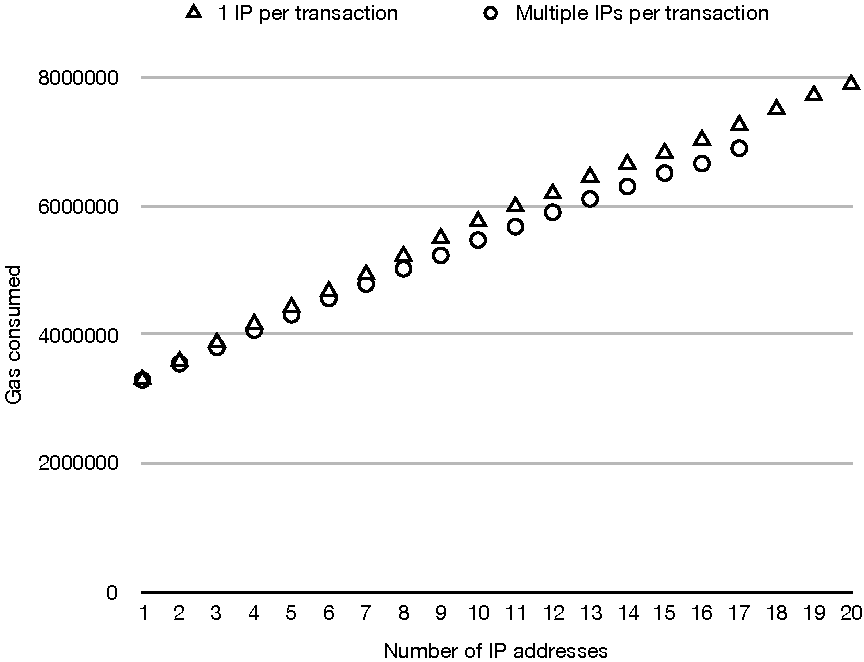
\includegraphics[width=0.7\textwidth]{v3-gas-cost.pdf}
\caption{Gas cost incurred using variant 3}
\label{fig:v3-gas-cost}
\end{figure}

\subsection{Variant 3}
For variant 3 (bloom filter variant), another benchmark script was created\footnote{The source code can be found under \texttt{v3-gas-benchmark.js}. The benchmark can be executed with \texttt{node index v3-gas-benchmark --count=5}.}. Like in variant 1, a worst case and a best case scenario was tested, where in the worst case one report gets added at a time, while in the best case, reports could be bundled into one transaction to save gas.

This variant was expected to perform better than variant 1, as less storage is required to store all IP addresses. However, the benchmark does not confirm the expectation. The bloom filter does actually incur more gas costs than storing a full-sized array of IP addresses. 

For adding one report, approximately 290'000 gas is consumed, which is almost three times more than in variant 1 (105'000 gas). There are also no economies of scale, as the cost goes up linearly after the first report. Bundling reports into one transaction does save approximately 40'000 gas per report (13\%), but is less effective than it is for variant 1. Also, it is not possible to add more than 17 reports in one transaction, as the block gas limit is reached.

It becomes clear that Solidity charges more heavily for expensive computation like hashing than it does for storage.
In addition to much higher costs, the bloom filter variant can also give false positives, and metadata like expiration date, whitelist/blacklist etc. has to be stored separately.

If less required storage space does not result in lower prices, then there is no advantage in it at all. The whole blockchain, multiple gigabytes needs to be downloaded to a client anyway \textemdash {} the only reason to optimize for storage is to get cheaper costs.

\section{Speed}

This thesis does pass on a speed benchmark. Current speed is dependant on several network parameter and can change over time. Additionally, by tweaking the amount of gas provided to a transaction the speed inserting reports is modifiable.

These factors make speed hard to quantify without some  assumptions about the network and the user preference. Instead, chapter 4 can be used as a reference for estimating the speed given assumptions. At the time of writing, the range of speeds that are possible is between 30 and 120 seconds. All Ethereum transactions fall inbetween these transaction times, therefore all variants are equally fast.

\section{Accuracy}

Variant 1 and 2 store the reports and the IP addresses in a lossless format, guaranteeing perfect accuracy. Variant 3 however does lose accuracy because of the bloomfilter, the exact amount of which is calculated in this section.

Given a number of items that are indexed, and a number of hash functions, the ideal array size and number of hash functions for a bloom filter can be calculated. According to \cite{BloomfilterAccuracy}, given $n$ = number of items in the filter and $p =$ probability of false positives, the number of bits in the filter $m$ can be calculated using equation \ref{eq:m} and the number of hash functions $k$ using equation \ref{eq:k}. 

\begin{equation}
m = \lceil\frac{n * log(p)}{ln(\frac{1.0}{2.0 ^{ln(2)}})}\rceil
\label{eq:m}
\end{equation}

\begin{equation}
k = \lfloor ln(2) * m / n) \rceil
\label{eq:k}
\end{equation}

For example: Given that the magnitude of DDoS attacks is in the millions (n = 1'000'000) and assuming that a 5\% chance of false positives is good enough (p = 0.05), an array size of 14357134 bits (1.71 MB) and 4 hash functions will do.

Solving equation \ref{eq:m} for $p$ gives equation \ref{eq:p}.

\begin{equation}
p = e^{\frac{{m \cdot ln(\frac{1}{2^{ln(2)}})}}{n}}
\label{eq:p}
\end{equation}

The probability of at least one false positive is shown in table \ref{table:Probability} and figure 5.3. It assumes the number of \textbf{bits} in the filter is 4'096 ($512\ bytes \cdot 8$).

\begin{table}[ht]
\begin{minipage}[b]{.45\textwidth}
        \begin{tabular}{r | r}
            \hline
            IP addresses ($n$) & Probability \\ \hline
            1 & $10^{-855}$ \\ \hline
            10 & $10^{-86}$ \\ \hline
            100 & $10^{-9}$ \\ \hline
            1'000 & 0.14 \\ \hline
            10'000 & 0.82 \\ \hline
            100'000 & 0.98 \\ \hline
            1'000'000 & 0.998 \\ \hline
            10'000'000 & 0.9998 \\ \hline
        \end{tabular}
            \caption{Probability of false positives, using equation \ref{eq:p} and $m = 4'096$}
            \label{table:Probability}
\end{minipage}
\hspace{.1\textwidth}
\begin{minipage}[b]{.45\textwidth}
        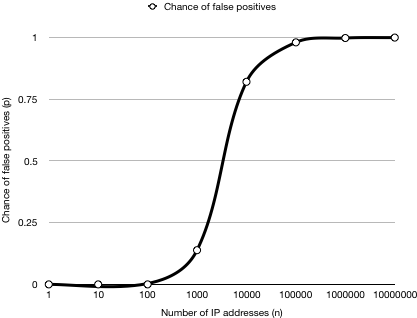
\includegraphics[width=1\textwidth]{v3-chance.png}
        \label{fig:Probability}
        \captionof{figure}{Probability of false positives, using data from Table \ref{table:Probability} (logarithmic scale)}
\end{minipage}
\end{table}

The bloom filter does have a false positive chance of under 1\% for up to 425 IP addresses. Inserting more IP addresses after that decreases the accuracy of the bloom filter dramatically. With 1'000 insertions, variant 3 would lead to 14\% of legimitate traffic being blocked. With 3'000 insertions, over half of the legitimate traffic would be falsly blocked.

With the gas limit constaint in place and the probabilities in mind, it is recommended to use more than one contract if the probability of false positives would be higher than acceptable otherwise. The acceptable probability of false positives is individual for each user.

